%\documentclass[aps,draft,showpacs]{revtex4-1}
%\documentclass[aps,pra,twocolumn,showpacs]{revtex4-1}
%\documentclass[aps,pra,showpacs]{revtex4-1}
%\documentclass[aps,prl,twocolumn,nofootinbib,showpacs]{revtex4}
\documentclass[aps,pra,twocolumn,showpacs]{revtex4-1}
\usepackage{amsbsy,latexsym,amsmath}
\usepackage{amsfonts}
\usepackage{amssymb}
\usepackage[mathscr]{eucal}
\usepackage{epsfig,graphics,graphicx}
\usepackage{color}
\usepackage{float}
%
%
%\documentclass[12pt]{article}
%\usepackage[english]{babel}
%\usepackage[applemac]{inputenc}
%\usepackage{graphicx}
%\usepackage{amsmath,amsthm,amsfonts,mathrsfs}
%\usepackage{verbatim}
%%\usepackage{fullpage}

%\setlength{\headsep}{20pt}
%\setlength{\textheight}{26.4cm}

\newcounter{saveenumi}
\parskip=1em


\newtheorem{lemma}{Lemma}

\begin{document}


 \title{Probabilistic Approximate Cloning}
\author{V. Yerokhin$^{1}$, A. Shehu$^{1}$, E. Feldman$^{2}$, E. Bagan$^{1,3}$ and J. A. Bergou$^{1}$}
\affiliation{$^{1}$Department of Physics and Astronomy, Hunter College of the City University of New York, 695 Park Avenue, New York, NY 10065, USA\\
$^{2}$Department of Mathematics, Graduate Center of the City University of New York, 365 Fifth Avenue, New York, New York 10016, USA \\
$^{3}$F\'{i}sica Te\`{o}rica: Informaci\'{o} i Fen\`{o}mens Qu\`antics, Universitat Aut\`{o}noma de Barcelona, 08193 Bellaterra (Barcelona), Spain
}

\begin{abstract} 
Boost up the success probability by allowing some degree of approximation. Linear optics implementation.  Asymptotic convergence to FRIO (measure and prepare). Phase transition at the unambiguous discrimination end.
\end{abstract}
\pacs{03.67.-a, 03.65.Ta,42.50.-p }
\maketitle 

Probabilistic protocols enable us to carry out tasks that are impossible deterministically according to the laws of quantum mechanics, thus opening new possibilities for the processing of quantum information and broadening the scope of  quantum technologies. Remarkable examples of this are unambiguous state discrimination, whereby non-orthogonal states can be identified without error; perfect cloning of a known set of states, which can be performed probabilistically whereas its deterministic version is forbidden by the no-cloning theorem. More recent advances include replication, amplification, probabilistic metrology.

The price to pay for making the impossible possible is that those protocols fail sometimes. To assess the amount of resources that a given task will require it is necessary to know what is the minimum failure probability $Q$ of the corresponding protocols. This minimum failure probability, or alternatively, the maximum success probability, often defines the optimal probabilistic protocol. A relevant practical question arises at this point, particularly, if the value of $Q$ turns out to be large. Can we increase the success probability by allowing small imperfections or a small number of errors? 



Here, we address this question for cloning. We will show that indeed approximate clones can be obtained for failure rates below the minimum failure rate $Q_{\rm PC}$ of perfect cloning.

benchmarks 

Perfect cloning vs approximate cloning 

Boost up the success probability by allowing some degree of approximation: FRIO 

Physical inplementation with linear optics 

\bigskip


A relevant practical question concerning unambiguous discrimination is if one can increase the probability of success, by allowing some small probability of error, smaller than the minimum probability of error of the deterministic discrimination protocol. The answer is known to be in the positive, and gives rise to a scheme that can be presented in different fashions. One can, e.g., set a margin on the individual error probabilities, or on the average error probability. Equivalently, one can set a margin on the average probability of inconclusive outcomes produced by the scheme.  The latter bears strong connections/links with the cloning scheme to which his paper is devoted. We will refer to it as Fix Rate of Inconclusive Outcome scheme, or FRIO scheme for short~\cite{FRIO}. 


\section{Results}

Global fidelity vs local fidelity.

Asymptotic convergence to FRIO (measure and prepare). 

Phase transition at the unambiguous discrimination end.

The physical implementation.

\bigskip
Without loss of generality, we will assume throughout the paper that $0\le\eta_1\le 1/2\le \eta_2\le 1$.
\bigskip

\noindent{\bf The optimal cloner.} We focus on $1\to n$ cloning for simplicity. For~\mbox{$m\to n$} cloning we just make the replacement $|\psi_k\rangle\to|\psi_k^m\rangle\equiv|\psi_k\rangle^{m}$.
We address optimality from a Bayesian viewpoint that assumes the two states to be cloned are given with some {\it a priori}  probabilities~$\eta_1$ and~$\eta_2$, so~$\eta_1+\eta_2=1$. Then a natural cost function for a probabilistic cloner is given by the average failure probability 
%
\begin{equation}
Q=\eta_1 q_1+\eta_2 q_2,
\label{obj fun}
\end{equation}
where $q_k$ is the failure probability if the state $|\psi_k\rangle\in{\mathscr H}$ is fed into the cloner. Let $|\Psi_k\rangle\in{\mathscr H}^{\otimes n}$, $k=1,2$, be the state of the~$n$ clones of $|\psi_k\rangle$. 
%Then, the average fidelity is
%% 
%\begin{equation}
%F=\eta_1|\langle \psi^n_1|\Psi_1\rangle|^2 +\eta_2|\langle \psi^n_2|\Psi_2\rangle|^2,
%\end{equation}
%%
%where $|\psi^n_k\rangle$ is the states of~$n$ perfect clones. 
%For a given $Q$, the optimal cloner is that for which the average fidelity is maximum.
Ideally, one would like the cloner to output perfect copies, i.e.,  $|\Psi_k\rangle=|\psi^n_k\rangle$. According to the no-cloning theorem this requires a minimum failure probability $Q_{\rm PC}>0$, where PC stands for perfect cloning. In this framework, optimal perfect cloning has been addressed and solved in full generality only very recently~\cite{us1}. Here we wish to find the optimal approximate cloner
for a given~$Q$ smaller than~$Q_{\rm PC}$. That is, the cloner that outputs the most approximate clones. The exact meaning

%
In this paper we will use an approach based on Neumark's theorem and characterize a cloner of the kind we have introduced by a unitary transformation $U$ acting on the input (in the state $|\psi_k\rangle$) and some conveniently chosen ancillary system. We assume that initially the ancilla is in a reference state $|0\rangle$. The transformation $U$ should render the system composed of the input and the ancilla in the state $|\Psi_k\rangle|s\rangle=|\Psi_k\rangle\otimes|s\rangle$ ($|\Phi\rangle|f\rangle=|\Psi_k\rangle\otimes|s\rangle$) in case of success (failure). Here, $|s\rangle$ and $|f\rangle$ refer to two orthogonal states of a part of the ancillary system that plays the role of a flag. By reading the state of the flag we know whether cloning has succeeded of failed. If cloning has failed, the output is in a failure state $|\Phi\rangle$. Optimality requires  $|\Phi\rangle$ to be one and the same regardless of the state fed into the cloner~\cite{us1,us2}. The above can be written as
%
\begin{eqnarray}
U|\psi_1\rangle|0\rangle&=& \sqrt{p_1}|\Psi_1\rangle|s\rangle +\sqrt q_1 |\phi\rangle|f\rangle,\label{U1}\\
U|\psi_2\rangle|0\rangle&=& \sqrt{p_2}|\Psi_2\rangle|s\rangle +\sqrt q_2 |\phi\rangle|f\rangle. \label{U2}
\end{eqnarray}
%
%Likewise, we could consider an even more general setup with two failure states $|\phi_1\rangle$ and $|\phi_2\rangle$ in Eqs.~(\ref{U1}) and~(\ref{U2}). This is necessarily sub-optimal since we could probabilistically determine whether we received $|{\psi_1}\rangle$ or $|{\psi_2}\rangle$ by applying unambiguous discrimination to the failure states~$| {\phi_k}\rangle$.  Sometimes we would be  certain of the input state, in which case we could  prepare $|\Psi_1\rangle$ or~$|\Psi_2\rangle$ accordingly,  thereby increasing the overall success rate.
%
Taking the inner product of Eqs.~(\ref{U1}) and ~(\ref{U2}) with themselves shows that our probabilities are normalized: $p_i+q_i=1$.
Similarly, by taking the product of Eq.~(\ref{U1}) with Eq.~(\ref{U2}), we find the unitarity constraint,
%
\begin{equation}
s=\sqrt{p_1 p_2}\, s'+\sqrt{q_1 q_2},
\label{unit cond}
\end{equation}
%
where $s\equiv|\langle\psi_1|\psi_2\rangle|$ and $s'\equiv|\langle\Psi_1|\Psi_2\rangle|$. Without any loss of generality, in deriving Eq.~(\ref{unit cond}) we have chosen
$\langle {\psi_1}|{\psi_2}\rangle$ and $\langle {\Psi_1}|{\Psi_2}\rangle$ to be real and positive.
If Eq.~(\ref{unit cond}) is satisfied, it is not hard to prove that~$U$ has a unitary extension on the whole Hilbert space

Following~\cite{Chefles+Barnett inter}, we asses the quality of the approximate clones  $|\Psi_k\rangle\in{\mathscr H}^{\otimes n}$, $k=1,2$ by means of the averaged global fidelity, which we will call just fidelity for brevity. The fidelity of the clones $|\Psi_k\rangle$ is $F_k=|\langle\psi_k^n|\Psi_k\rangle|^2$. If the cloner is fed with the state $|\psi_k\rangle$, it successfully delivers~$|\Psi_k\rangle$ with probability $p_k$ and fails with probability~$q_k=1-p_k$. The probability of delivering~$|\Psi_k\rangle$ is then~$\eta_k p_k$ and the total success (failure) probability is $\bar Q=\eta_1p_1+\eta_2p_2$ ($Q=1-\bar Q=\eta_1q_1+\eta_2q_2$). Throughout the paper, we will use the notation $\bar x=1-x$ for any quantity $x$. The average probability (conditioned to successfully cloning the input state) is then %$F=(\eta_1p_1F_1+\eta_2p_2 F_2)/P$.
%
\begin{equation}
F=\tilde\eta_1|\langle \psi^n_1|\Psi_1\rangle|^2 +\tilde\eta_2|\langle \psi^n_2|\Psi_2\rangle|^2,
\end{equation}
%
where $\tilde\eta_k\equiv \eta_kp_k/\bar Q$ are the posterior probabilities conditioned to success. We readily have $\tilde\eta_1+\tilde\eta_2=1$. We can use Eq.~(\ref{F_max}) in Methods to write
%
\begin{equation}
F_{\rm max}={1\over2}+{1\over2}
\sqrt{\!1-\!4\tilde\eta_1\tilde\eta_2\sin^2(2\theta\!-\!2\theta')} .
\end{equation}
%
where
%
\begin{equation}
\cos2\theta=s^n,\quad \cos2\theta'=s' .
\label{thetas-overlaps}
\end{equation}
%
This equation can be written as
%
\begin{equation}
F_{\rm max}={\bar Q+\sqrt{\bar Q^2-4\eta_1\eta_2\zeta^2}\over2\bar Q} ,
\label{Fmax}
\end{equation}
%
where we have defined $\zeta\ge0$ as
%
\begin{equation}
\zeta=\sqrt{p_1p_2}\sin(2\theta-2\theta').
\end{equation}
%
The original overlap $s$ is given, but the overlap of the final states, $s'$ is not. It must be optimized so that the fidelity is maximized. This is, naturally, equivalent to minimizing~$\zeta$.
We can ged rid of trigonometric functions in the definition of~$\zeta$ by using Eq.~(\ref{thetas-overlaps}). This leads to
%
\begin{equation}
\zeta=\sqrt{p_1p_2}s'\sqrt{1\!-\!s^{2n}}\!-\!s^n\sqrt{p_1p_2(1\!-\!s'^2)} .
\label{zeta notrig}
\end{equation}
%
We can now use the unitarity constraint, Eq.~(\ref{unit cond}), to get rid of $s'$ and write
%
\begin{equation}
\zeta\!=\!(s-\sqrt{q_1q_2})\sqrt{1\!-\!s^{2n}}\!-\!s^n\!\sqrt{p_1p_2\!-\!(s\!-\!\sqrt{q_1q_2})^2},
\end{equation}
%
or equivalently,
%
\begin{eqnarray}
\zeta&=&(s-\sqrt{q_1q_2})\sqrt{1-s^{2n}}\nonumber\\
&-&s^n\sqrt{1-s^2+2\sqrt{q_1q_2}s-(q_1+q_2)},
\label{zeta-means}
\end{eqnarray}
%
which is a function of the arithmetic and geometric means of the failure probabilities $q_1$ and $q_2$ alone. We note that~$\zeta$ is also independent of the priors $\eta_1$ and $\eta_2$.
The original optimization problem is now cast as
%
\begin{eqnarray}
&\displaystyle \min_{0\le q_1,q_2\le1} \zeta,&\nonumber\\[.5em]
&\mbox{\rm subject to}&\nonumber\\[.5em]
&\mbox{$\displaystyle Q=\eta_1 q_1+\eta_2 q_2$ and $\zeta\ge0$}.&
\end{eqnarray}
%
If $q^*_k$ are the values of $q_k$ that minimize $\zeta$ and $p^*_k=1-q^*_k$, then the overlap of the output states is
%
\begin{equation}
s'={s-\sqrt{q^*_1q^*_2}\over\sqrt{p^*_1p^*_2}}.
\end{equation}
%

\bigskip

\noindent{\bf Geometrization of the problem.} Eq.~(\ref{zeta-means}) suggest that the geometric and arithmetic means of the failure probabilities $q_1$ and $q_2$ should be a good set of variables. So, following Ref.~\cite{us2}, let us define
%
\begin{equation}
u=\sqrt{q_1q_2},\quad v={q_1+q_2\over2}.
\label{u-v def}
\end{equation}
%
Before discussing the geometric features of Eq.~(\ref{zeta-means}) in terms of these new variables, it it convenient to recall how the map in Eq.~(\ref{u-v def}) acts on~Eq.~(\ref{obj fun})~\cite{us2}. It is not hard to see that
this straight line maps into the ellipse
%
\begin{eqnarray}
u&=&{Q\over\sqrt{1-\Delta^2}}\cos\phi,\nonumber\\
v&=&{Q\over1-\Delta^2}+{Q\Delta\over1-\Delta^2}\sin\phi,
\label{obj fun conic}
\end{eqnarray}
%
where we have defined $\Delta=\eta_2-\eta_1$.  We readily see that the eccentricity of the ellipse is only a function of the priors. For equal priors, $\Delta=0$, the ellipse degenerates into the horizontal segment $v=Q$, $0\le u\le Q$, whereas for $Q=0$ it collapses into the origin $(u,v)=(0,0)$. As one increases $Q$, a family of similar ellipses is obtained. As they increase in size, their center moves up along the~$v$ axis. The line $u=v$ is the envelope of this family, as one can easily check using~Eq.~(\ref{obj fun conic}).

%
\begin{figure}[t]
\centering
$%
\begin{array}{c}
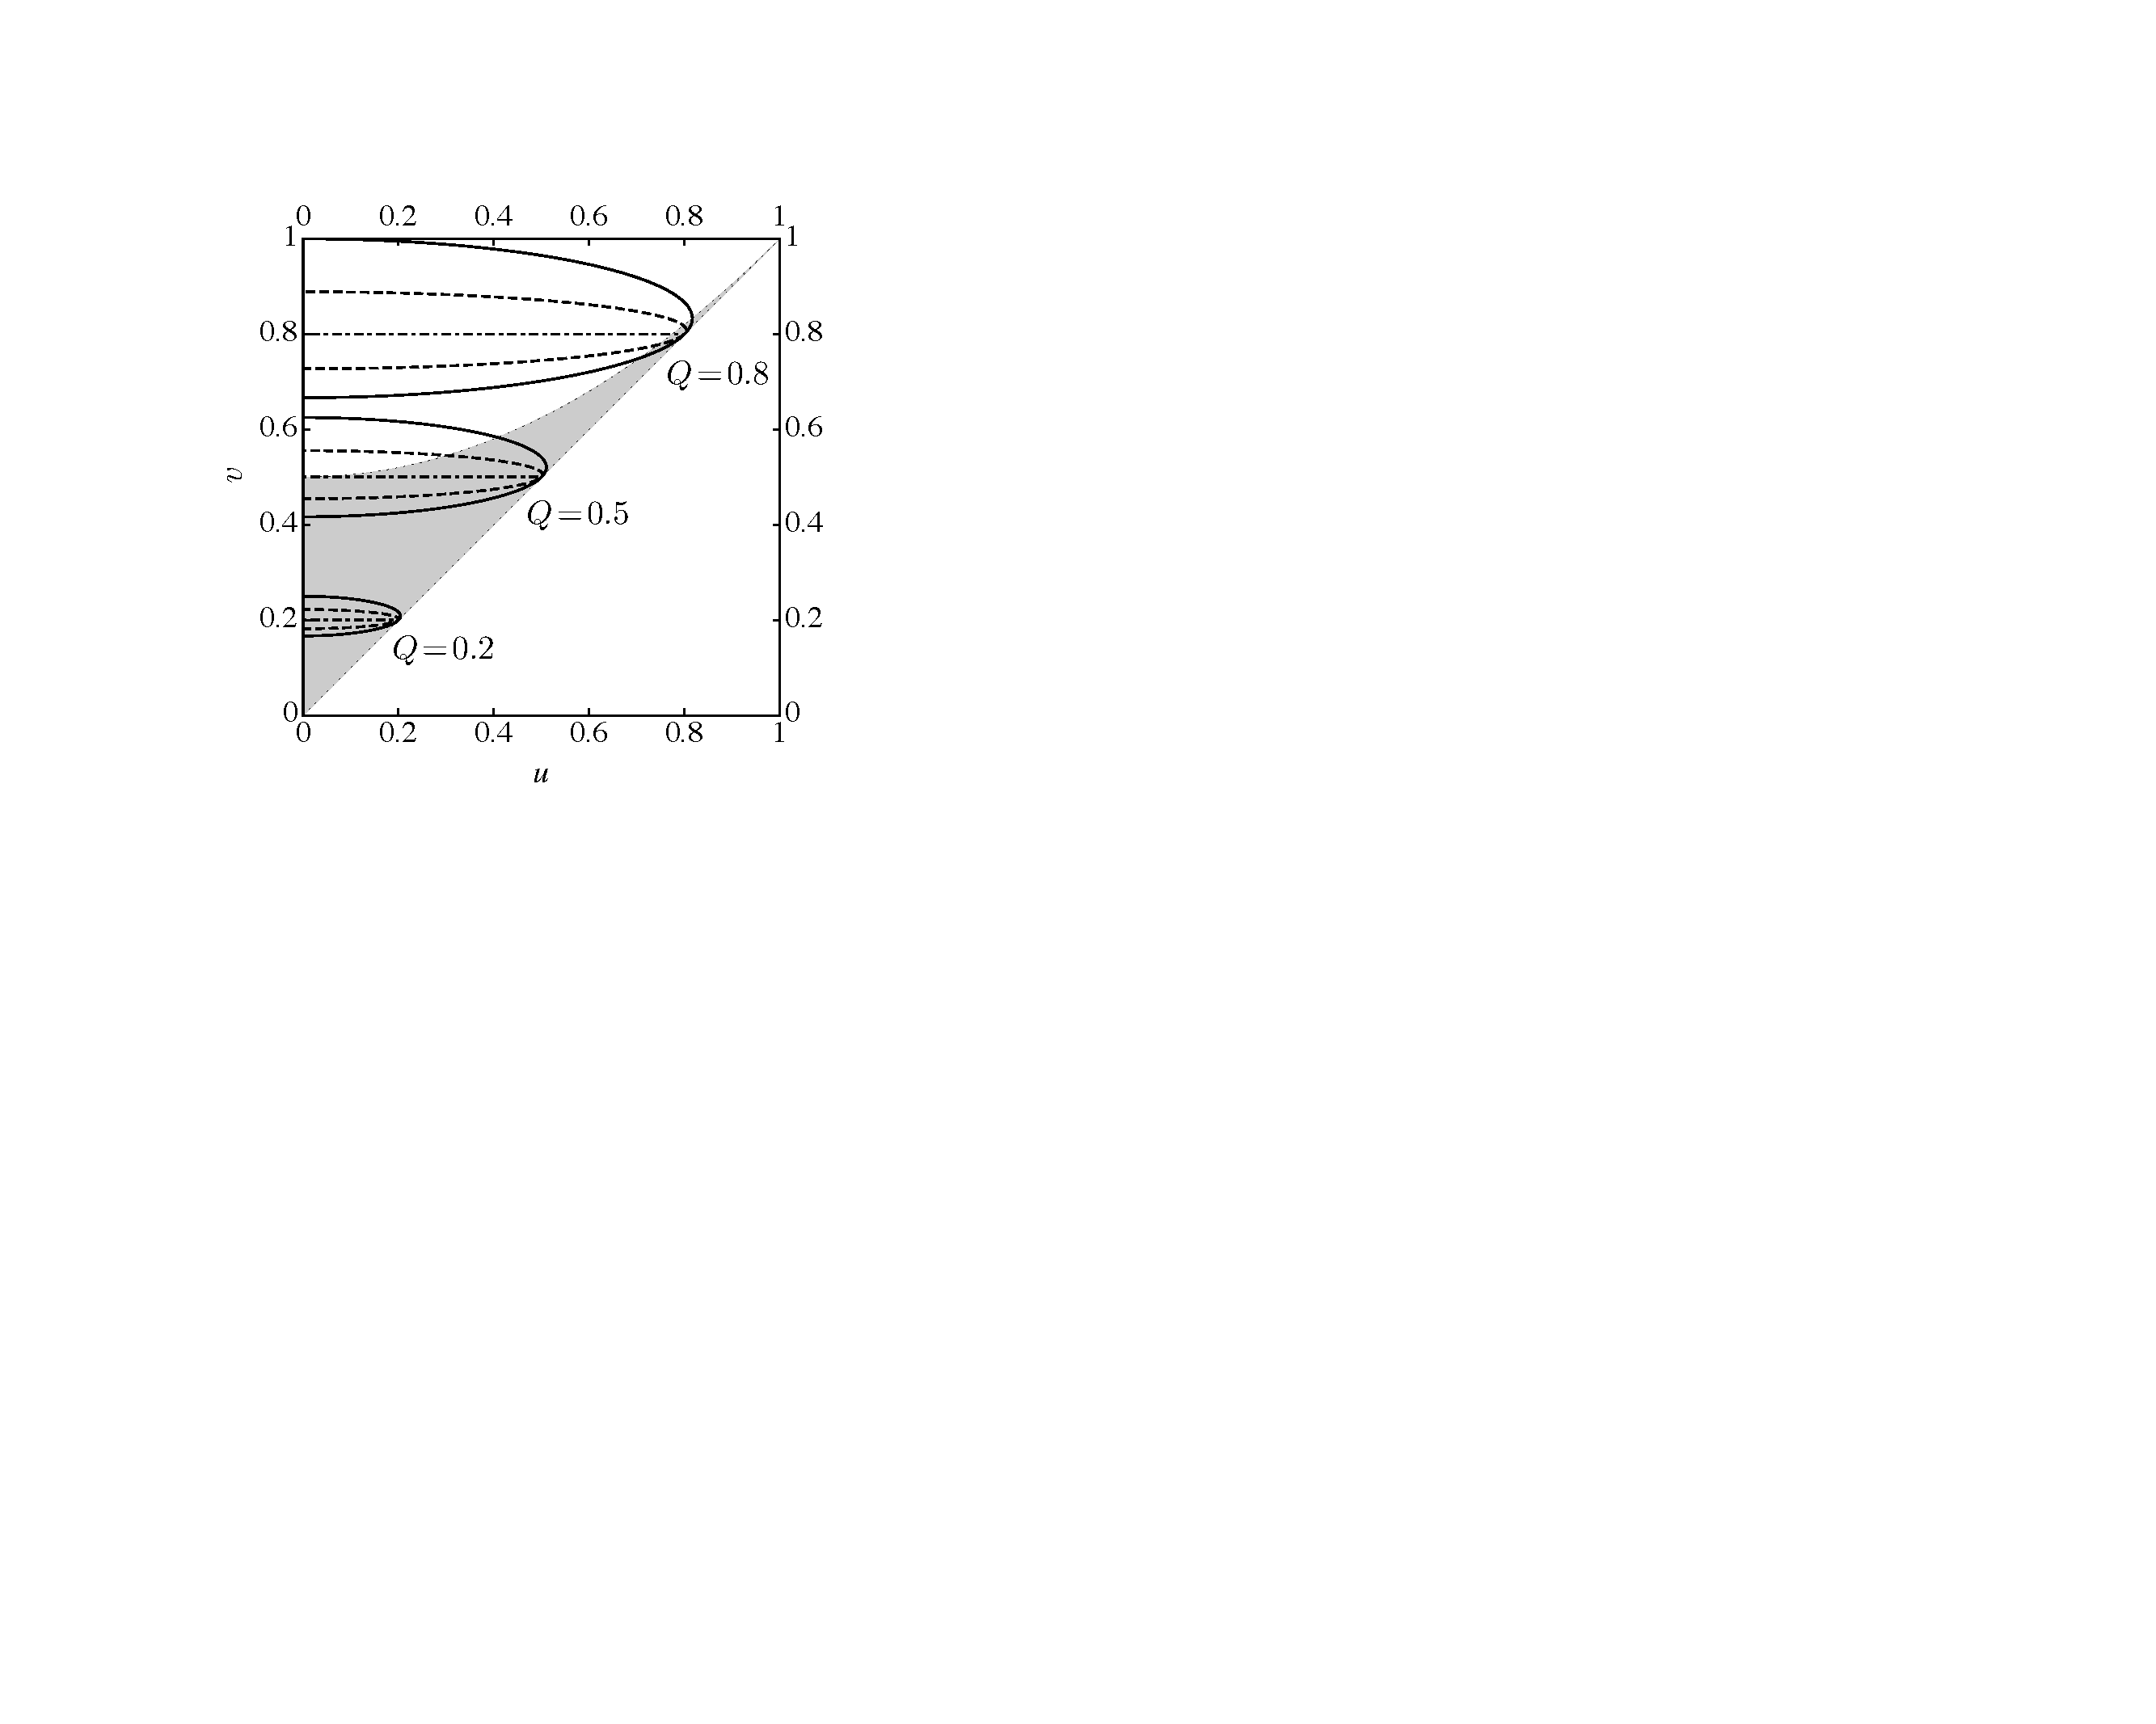
\includegraphics[width=16em]{ApproximateClones_F2b.pdf}\\
\end{array}%
$%
\caption{The ellipses in Eq.~(\ref{obj fun conic}) for various values of the failure rate $Q$ and for $\Delta=0.2$ (solid line), $\Delta=0.1$ (dashed lines). The bottom boundary line to the gray region, i.e., the straight line~$v=u$, is the envelope of these families of ellipses. The geometric solution to optimal cloning falls in the gray region. The degenerate ellipses for $\Delta=0$ (dot-dashed lines) are also shown.}
\label{fig:ellipses}
\end{figure}
%

We now turn to Eq.~(\ref{zeta-means}). In term of the new variables~$u$ and~$v$, this equation becomes the parabola
%
\begin{equation}
v=su+{1\!-\!s^2\over2}-{1\!-\!s^{2n}\over2s^{2n}}\left(\!u\!-\!s+{\zeta\over\sqrt{1\!-\!s^{2n}}}\right)^2\kern-.2em.
\label{para}
\end{equation}
%
If $\zeta=0$, Eq.~(\ref{para})  can be also written as
%
\begin{equation}
v={1+u^2\over2}-{(u-s)^2\over2s^{2n}}.
\label{para z=0}
\end{equation}
%
As $s$ varies from $0$ to unity, this equation describes a family of parabolas whose envelope is also a parabola, given by the first term of Eq.~(\ref{para z=0}). For $s=0$, the parabola degenerate into a straight vertical segment of height $1/2$ at~$u=0$. The parabolas become wider as $s$ increases. Eq.~(\ref{para z=0})~agrees with Eq.~(16) in~\cite{us2} if the overlap of the output states is $s'=s^n$. This is the overlap of $n$ perfect clones, as it should be, since $\zeta=0$ implies $F_{\rm max}=1$. By increasing $n$, the parabolas described by Eq.~(\ref{para z=0}) become narrower. In the limit $n\to\infty$, they degenerate into vertical straight segments at $u=s$ of height $(1+s^2)/2$. Some of there features are illustrated in Fig.~\ref{fig:const z}~(a).
 
Because of the way we have written Eq.~(\ref{para}), it is apparent that for fixed input overlap $s$, the envelope of the family of parabolas obtained as $\zeta$ varies is the straight line given by the first two terms on the right hand side of Eq.~(\ref{para}), namely,
%
\begin{equation}
v=su+{1-s^2\over2}.
\label{env par}
\end{equation}
%
As $\zeta$ increase from its minimum value, $\zeta=0$, the parabolas slide down along this straight line, Eq.~(\ref{env par}), without distortion. Since any physically realizable cloner with failure probability $Q$ corresponds to a point $(u,v)$ that belongs to both, an ellipse and a parabola, for a given~$s$ and~$Q$, the optimal solution is given by the value of $\zeta$ that makes the parabola tangent to the ellipse. We see~that the upper end of the allowed $\zeta$ interval cannot exceed $\zeta_{\rm max}=s\sqrt{1-s^{2n}}-s^n\sqrt{1-s^2}$. This is the value of $\zeta$ for which the corresponding parabola contains the origin $(u,v)=(0,0)$, i.e., gives the solution for the deterministic cloner ($Q=0$). By increasing $n$ we make the parabolas narrower. In the limit $n\to\infty$, they become a vertical segment of height $(1+s^2)/2-s\zeta$ at the point~$u=s-\zeta$.

%
\begin{figure}[t]
\centering
$%
\begin{array}{c}
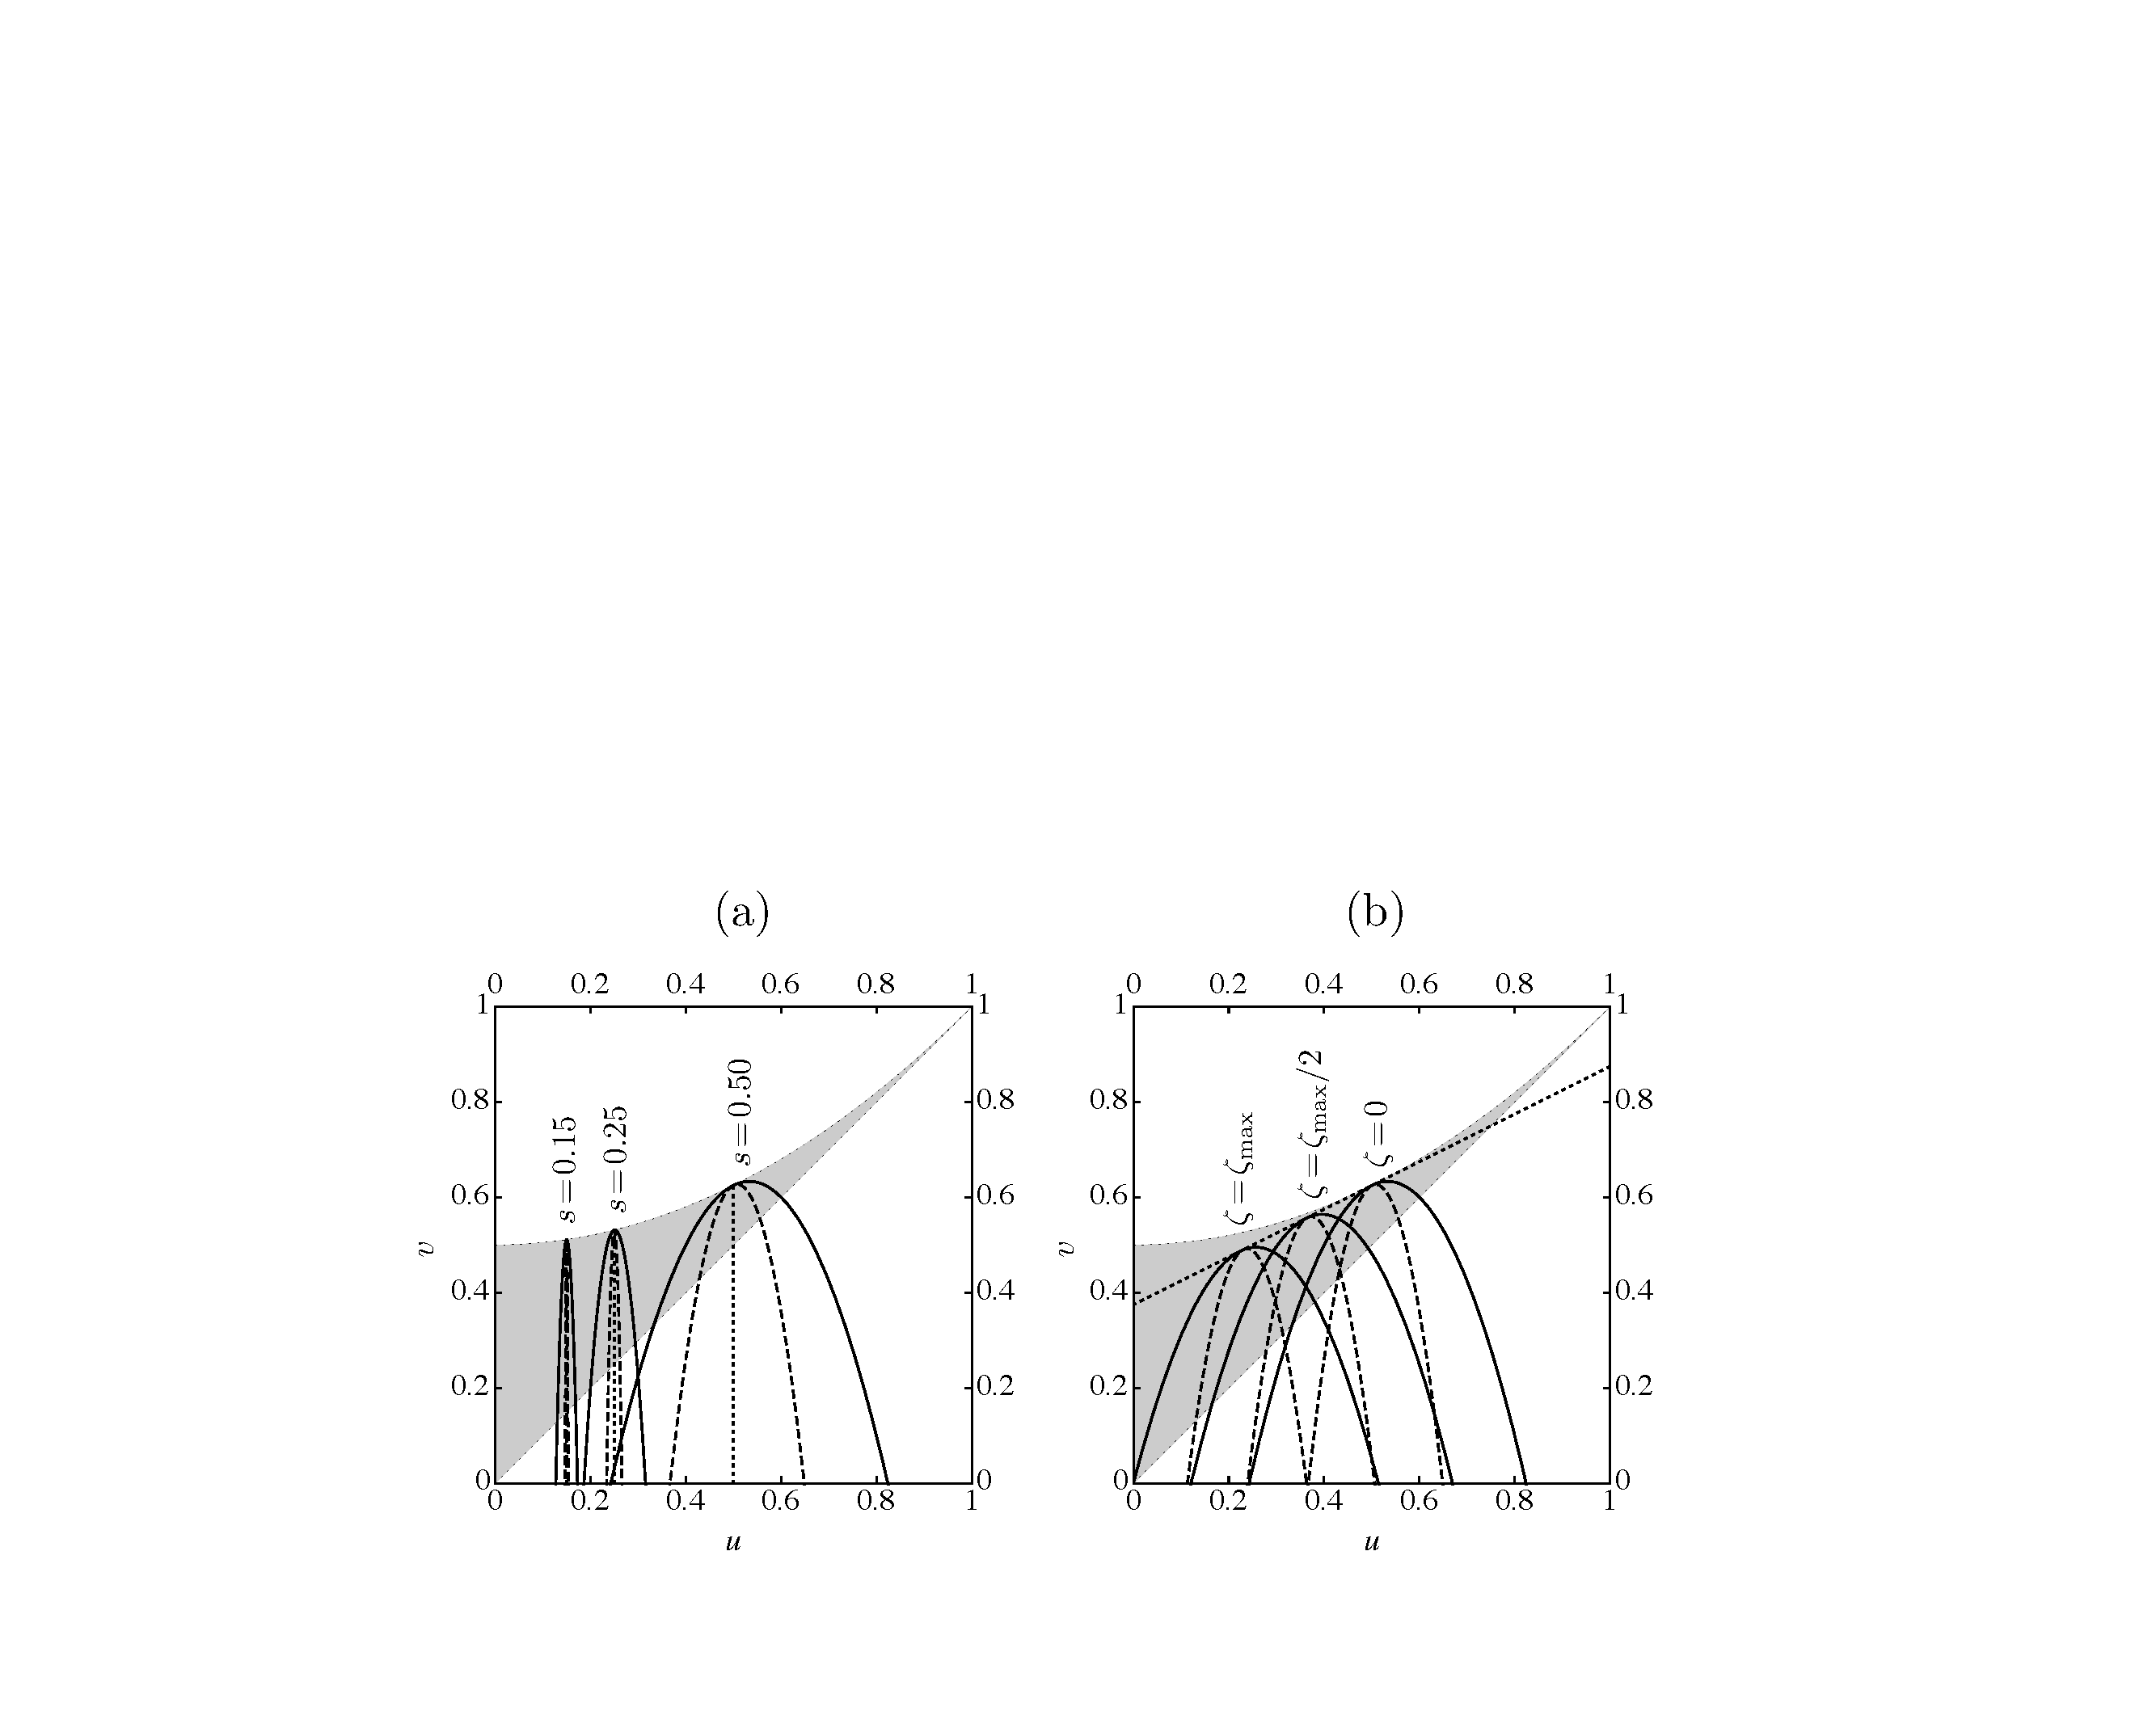
\includegraphics[width=26em]{ApproximateClones_F3.pdf}\\
\end{array}%
$%
\caption{(a) Parabolas defined by Eq.~(\ref{para z=0}) for different values of~$s$ and $n=2$ (solid lines) and $n=3$ (dashed lines). The dotted lines correspond the degenerate case of $n\to\infty$. The~top boundary line to the gray region, given by $v=(1+u^2)/2$, is the envelope of these families of parabolas.  (b) Families of parabolas defined by Eq.~(\ref{para}) for fixed $s$ (in the figure~$s=0.5$) and various values of $\zeta$, $n=2$ (solid line) and~$n=3$ (dashed line). The value of $\zeta_{\rm max}$, computed for the solid-line family, is~$\zeta^{(n=2)}_{\rm max}=0.268$. For the dashed-line family, $\zeta^{(n=3)}_{\rm max}=0.388$. The dotted straight line is the envelope of these families of parabolas, obtained by varying~$\zeta$.}
\label{fig:const z}
\end{figure}
%
 

Ideally, we would like to find the optimal solution by computing the point of tangency between the conics we have just introduced. Unfortunately, this involves solving higher degree polynomial equation for which no formula for the roots exists. We therefore proceed as in~\cite{us2} and find the curve $F_{\max}(Q)$ in parametric form. The solution is (see Methods)
%
\begin{eqnarray}
Q\!&=&\!{(1\!-\!\Delta^2)(1\!-\!s^2)\!-\!\gamma_n\left(\Delta\cot\phi\!+\!s\sqrt{1\!-\!\Delta^2}\right)^2\over2\left(1+\Delta\sin\phi-s\sqrt{1-\Delta^2}\cos\phi\right)},
\nonumber\\
%\zeta \!&=&\!{1\over\sqrt{1+\gamma_n}}\left[(1\!+\!\gamma_n)s\!+\!{\gamma_n\Delta\cot\phi\over\sqrt{1\!-\!\Delta^2}}\!-\!{Q\cos\phi\over\sqrt{1\!-\!\Delta^2}}\right]
\zeta \!&=&\!{(1\!+\!\gamma_n)\sqrt{1\!-\!\Delta^2}s\!+\!\gamma_n\Delta\cot\phi\!-\!Q\cos\phi\over\sqrt{1+\gamma_n}\sqrt{1\!-\!\Delta^2}},
\label{sol par}
\end{eqnarray}
%
where $\gamma_n=s^{2n}/(1-s^{2n})$. We have $\lim_{n\to\infty}\gamma_n=0$. The upper end of the $\phi$ interval is given by the deterministic limit $Q=0$. This gives 
%
\begin{equation}
\cot\phi_{\rm max}=-\left(s+\sqrt{{1-s^2\over \gamma_n}}\;\right){\sqrt{1-\Delta^2}\over\Delta}
\end{equation}
%
The lower end of the interval is determined by perfect cloning, i.e., $F_{\rm max}=1$, which in turn imply~$\zeta=0$ and $s'=s^n$ [see, e.g., Eqs.~(\ref{thetas-overlaps}) or~(\ref{zeta notrig})]. However, no closed formula exists for~$\phi_{\rm min}$ and it value has to be computed numerically.  For smaller values of $\phi$, Eq.~(\ref{sol par}) does not give the optimal solution. These values would lead to failure probabilities larger than that required for perfect cloning. The strategy defined by Eq.~(\ref{sol par}) would produce separations below that required by perfect cloning, until full separation, $s'=0$ is attained. For this range of $Q$, the optimal scheme is perfect probabilistic cloning.

Combining Eq.~(\ref{Fmax}) with Eq.~(\ref{sol par}) we obtain the tradeoff curve $F_{\rm max}(Q)$. Examples for different values of can be found in Fig.~\ref{fig:tradeoff}.

%
\begin{figure}[t]
\centering
$%
\begin{array}{c}
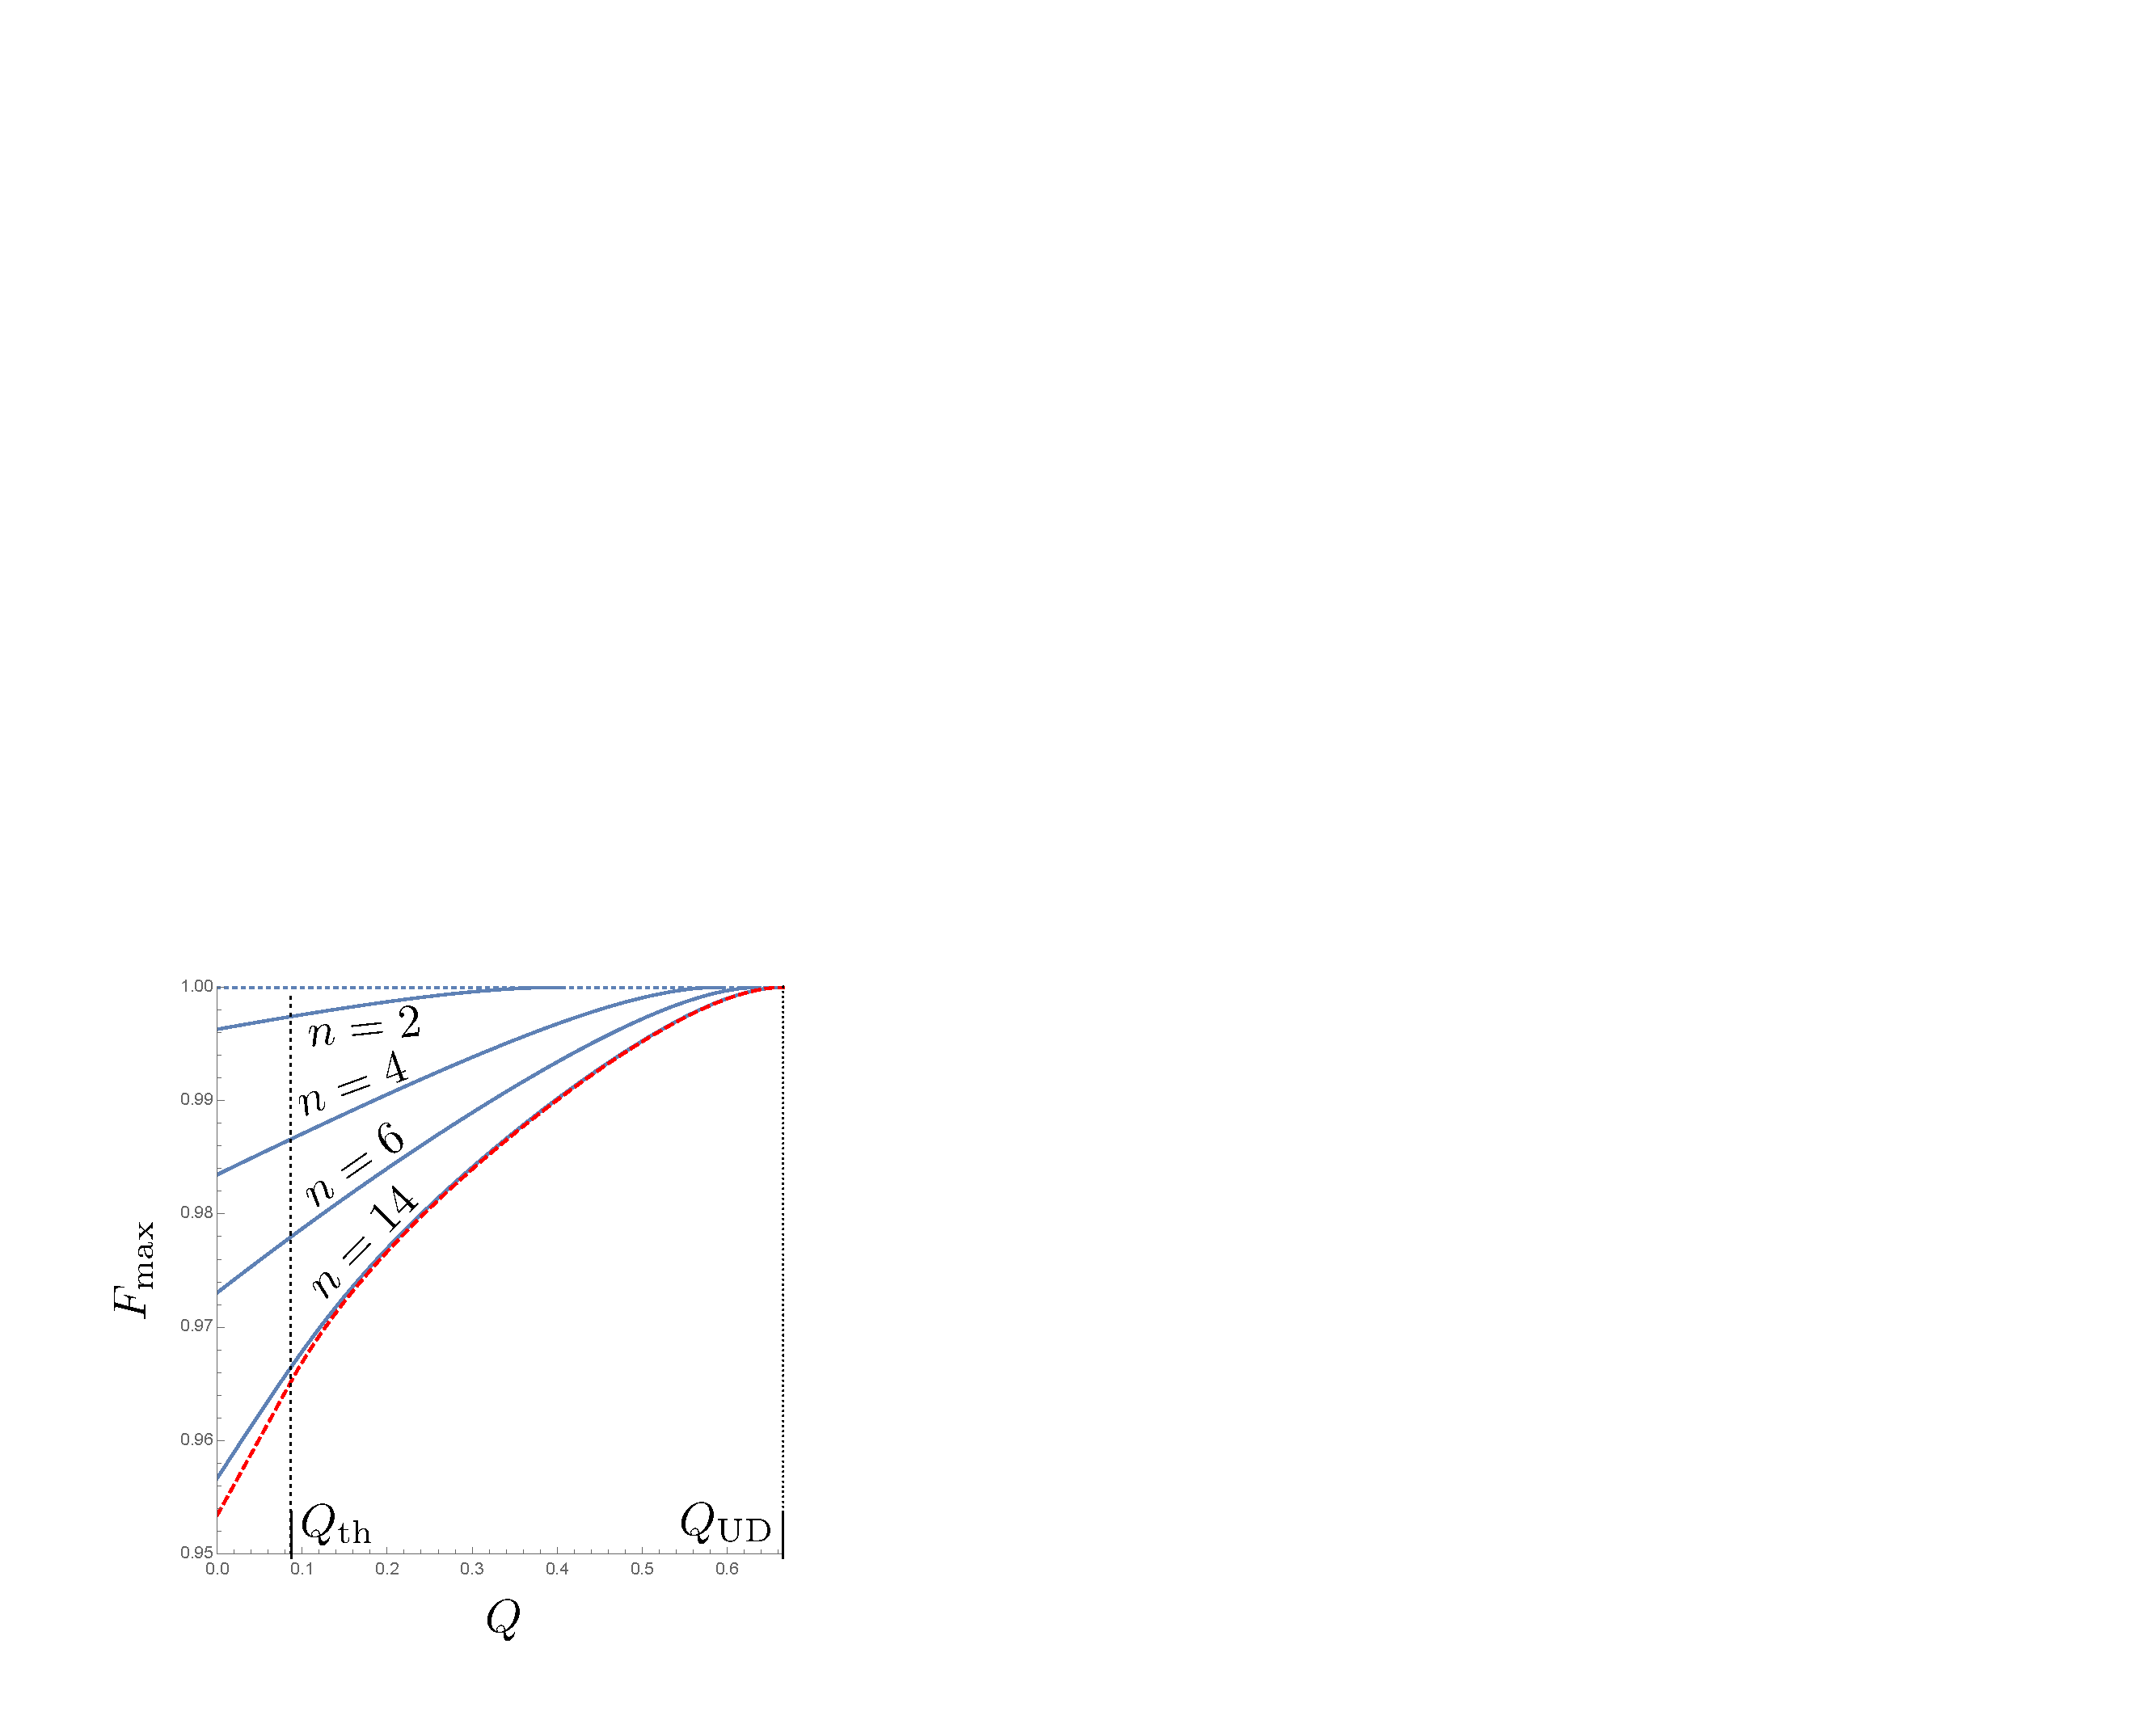
\includegraphics[width=16em]{ApproximateClones_F1.pdf}\\
\end{array}%
$%
\caption{ $F_{\rm max}$ vs $Q$ in the range $[0,Q_{\rm UD}]$ for various values of~$n$ and $s=0.8$, $\Delta=0.85$. A vertical (dotted) line is drawn at the threshold falure rate $Q_{\rm th}$, at which the FRIO scheme (dashed line) changes regime. The lines attain the value $F_{\rm max}=1$ (perfect cloning) at $Q=Q_{\rm PC}$, given in Ref.~\cite{us1}. The lines approach the FRIO line, whose second derivative is discontinuous at $Q=Q_{\rm th}$, as $n$ becomes larger. All the lines are have continuous derivatives for finite $n$.}
\label{fig:tradeoff}
\end{figure}
%

\bigskip

\noindent{\bf Asymptotic limit of many clones.} This limit is of fundamental importance. We show that as $n\to\infty$, the optimal protocol in measure and prepare. More precisely, the optimal cloning protocol can be implemented as a FRIO discrimination of the input states followed by a preparation of $|\psi^n_k\rangle$ if the discrimination is conclusive. The fidelity (conditioned on a conclusive identification) for such protocol is 
%
\begin{equation}
F=\eta_1{p_1+r_1 s^{2n}\over\bar Q}+\eta_2{p_2+r_2 s^{2n}\over\bar Q}
\end{equation}
%
where $p_k$ ($r_k$) is the probability of (mis)identifying the input state $|\psi_k\rangle$. If $n\to\infty$, we have $F^{\infty}=\tilde P_{\rm s}$, where~$\tilde P_{\rm s}$ is the FRIO success average probability condition on conclusive outcomes. 

Using the results  in~\cite{FRIO}, one can write
%
\begin{equation}
\tilde P_{\rm s}={\bar Q+\sqrt{\bar Q^2-(Q-Q_0)^2}\over2\bar Q},
\label{tildeP POVM}
\end{equation}
%
where 
$Q_0=2\sqrt{\eta_1\eta_2}s$ is the inconclusive (failure) probability for UD when $\eta_1\in[s^2/(1-s^2),1/2]$. For $\eta_1$ in this range, Eq.~(\ref{tildeP POVM}) holds for any meaningful value of the inconclusive probability $Q$, i.e., for $0\le Q\le Q_{\rm UD}=Q_0$. However, if the prior probabilities are very unbalanced, $\eta_1\in[0,s^2/(1-s^2)]$, two regimes exist. Eq.~(\ref{tildeP POVM}) holds only if $Q\le Q_{\rm th}$, where the threshold inconclusive probability is
%
\begin{equation}
Q_{\rm th}={2\eta_1\eta_2(1-s^2)\over 1-Q_0}.
\label{Q_th}
\end{equation}
%
For $Q_{\rm th}\le Q\le Q_{1}=\eta_1+\eta_2 s^2$, where $Q_{\rm UD}=Q_1$ in the above $\eta_1$ range, the three-outcome POVM protocol cannot be implemented and the optimal measurement is projective (two-outcome). Using the results in~\cite{FRIO} one can derive the expression 
%
\begin{equation}
\tilde P_{\rm s}={\eta_2\over\bar Q}{(\eta_2-\eta_1)(\eta_2-Q)c^2+\bar Q s^2+2\eta_1 sc R\over1-4\eta_1\eta_2c^2},
\label{tildeP proj}
\end{equation}
%
where $\bar Q=1-Q$, $c=\sqrt{1-s^2}$ and $R=\sqrt{Q\bar Q-\eta_1\eta_2 c^2}$. 

Now that we have given the relevant FRIO results we come back to computing the asymptotic limit of our cloning scheme.  To do that, we use our geometric picture. Since the parabolas in Eq.~(\ref{para}) become vertical segments in this limit, we notice that two different regimes will arise depending on whether the vertex of the ellipses in Eq.~(\ref{obj fun conic}) fall under the envelope (straight line) in Eq.~(\ref{env par}). The threshold is determined by the condition that the vertex ($\theta=0$) belongs to the envelope, i.e., satisfies Eq.~(\ref{env par}). We have
%
\begin{equation}
{Q_{\rm th}\over1-\Delta^2}=s{Q_{\rm th}\over\sqrt{1-\Delta^2}}+{1-s^2\over2}.
\end{equation}
%
Solving for $Q_{\rm th}$ we readily obtain Eq.~(\ref{Q_th}). For values of~$Q$ below the threshold, the corresponding ellipse and the vertical segment, located at $u=s-\zeta$, become tangent at the vertex, $\theta=0$, therefore $Q/\sqrt{1-\Delta^2}=s-\zeta$. This equation can be written as 
%
\begin{equation}
2\sqrt{\eta_1\eta_2}\zeta=Q_0-Q.
\end{equation}
%
Substituting this into Eq.~(\ref{Fmax}) we obtain the expression on the right hand side of Eq.~(\ref{tildeP POVM}).  For~$Q_{\rm th}\le Q$, the ellipse and the straight segment cannot be tangent. The ellipse merely touches the top of the vertical segment, so
%
\begin{eqnarray}
{Q\over\sqrt{1\!-\!\Delta^2}}\cos\phi\!&=&\!s\!-\!\zeta,\\
{Q\over1\!-\!\Delta^2}\!+\!{Q\Delta\over1\!-\!\Delta^2}\sin\phi\!&=&\!{sQ\over\sqrt{1\!-\!\Delta^2}}\cos\phi+\!{1\!-\!s^2\over2}.
\end{eqnarray}
%
We can solve the second equation for $\cos\phi$ to obtain
%
\begin{equation}
\cos\phi=\sqrt{1\!-\!\Delta^2}\,{s[2Q\!-\!(1\!-\!\Delta^2)c^2]\!+\!2\Delta c R\over2Q(s^2\!+\!\Delta^2 c^2)}.
\end{equation}
%
Substituting in the first equation we also have
%
\begin{equation}
\zeta={s[2(\Delta^2\!-\!Q^2)\!+\!(1\!+\! s^2)(1\!-\!\Delta^2)]\!-\!2\Delta c R\over2(s^2\!+\!\Delta^2 c^2)}.
\end{equation}
%
Substituting this in turn into Eq.~(\ref{Fmax}) we obtain (see details in Methods) the expression on the right hand side of Eq.~(\ref{tildeP proj}). In summary, $F^{\infty}_{\rm max}=\lim_{n\to\infty }F_{\rm max}=\tilde P_{\rm s}$ for all meaningful values of $Q$. Therefore, as anticipated, in the asymptotic limit of many copies optimal cloning can be implemented by FRIO discrimination followed by state preparation. 




%\bigskip
%
%\noindent{\bf Asymptotic limit of many clones (2).} This limit is of fundamental importance. From Eq.~(\ref{zeta-means}), it follows that $\lim_{n\to\infty}\zeta=s-\sqrt{q_1q_2}$. Substituting into Eq.~(\ref{Fmax}), we find
%%
%\begin{equation}
%F^\infty_{\rm max}={1-Q+\sqrt{(1-Q)^2-4\eta_1\eta_2(s-\sqrt{q_1q_2})^2}\over2(1-Q)}.
%\label{Fmax asym}
%\end{equation}
%%
%This expression must still be maximized over the failure probabilities $q_1$ and $q_2$. The right hand side is formally identical to the success probability of the discrimination protocol discussed in~\cite{FRIO}, where a Fixed Rate of Inconclusive Outputs (FRIO), $Q$, is allowed. More precisely, it is formally identical to $\tilde P_{\rm s}=P_{\rm s}/(1-Q)$. The maximization of Eq.~(\ref{Fmax asym}) is carried out in detail in the the Sec. Methods. It shows that the optimal scheme may have two distinct regimes depending on the values of the prior probabilities $\eta_1$, $\eta_2$. In particular, if $s^2/(1-s^2)\le\eta_1\le1/2$, then a three-outcome measurement scheme is optimal and the maximum success probability, conditioned to a conclusive outcome, is
%%
%\begin{equation}
%\tilde P_{\rm s}={1-Q+\sqrt{(1-Q)^2-(Q-Q_0)^2}\over2(1-Q)}.
%\label{tildeP POVM 2}
%\end{equation}
%%
%However, if the prior probabilities are very unbalanced, \mbox{$\eta_1\le s^2/(1-s^2)$}, the three-outcome measurement can only exists if $0\le Q\le Q_{\rm th}$, where
%%
%\begin{equation}
%Q_{\rm th}={2\eta_1\eta_2(1-s^2)\over 1-Q_0}.
%\end{equation}
%%
%In this case Eq.~(\ref{tildeP POVM}) still holds. For $Q_{\rm th}<Q\le Q_{\rm UD}$, only a projective measurement can exist and the success probability can implicitly be given by
%%
%\begin{equation}
%\sqrt{1-\tilde P_{\rm s}\over\eta_1}=s\sqrt{\tilde P_{\rm s}\over\eta_2}-\sqrt{1-s^2}\sqrt{{1\over1-Q}-{\tilde P_{\rm s}\over\eta_2}}.
%\end{equation}
%%
%This equation can be solved for $\tilde P_s$, but the final expression is cumbersome and we do not give it here. 

\section{Discussion}

...

\section{Methods}

\noindent{\bf Maximum fidelity.} For the sake of completeness, we here re-derive the maximum (global) fidelity of the deterministic cloning protocol. We follow Barnett and Chefles' derivation~\cite{Chefles+Barnett inter}, with slight modifications. We stick to our notation and recall that $|\Psi_k\rangle\in{\mathscr H}^{\otimes n}$ ($k=1,2$) is the state of the~$n$ approximate copies of $|\psi_k\rangle$, with prior probabilities $\eta_k$. Then, the average fidelity is
%
\begin{equation}
F=\eta_1|\langle \psi^n_1|\Psi_1\rangle|^2 +\eta_2|\langle \psi^n_2|\Psi_2\rangle|^2,
\end{equation}
%
where we recall that  $|\psi^n_k\rangle=|\psi_k\rangle^{\otimes n}$, i.e., $|\psi^n_k\rangle$ is the states of~$n$ perfect clones. The optimal cloner is that for which the average fidelity is maximum.
%Let $s$ and $s'$ be the overlaps of the initial (we consider $1\to n$ cloning for simplicity) and final states:
%$$
%s=\langle\psi_1|\psi_2\rangle,\qquad  s'=\langle\Psi_1|\Psi_2\rangle .
%$$
%For perfect clonig, we necessarily must have $s'=s^n$.
%The unitarity conditions imply that  %(we choose the optimal setup $\alpha=\phi=1$)
%$$
%s=s'\sqrt{p_1 p_2}+\sqrt{q_1q_2}.
%$$

With no loss of generality we may write
%
\begin{eqnarray}
|\psi^n_k\rangle&=&\cos\theta\,|0\rangle-(-1)^k\sin\theta\,|1\rangle,\nonumber\\
|\Psi_k\rangle&=&\cos\theta'\,|0'\rangle-(-1)^k\sin\theta'\,|1'\rangle,
\end{eqnarray}
%
where $\{|0\rangle,|1\rangle\}$ and $\{|0'\rangle,|1'\rangle\}$ are two conveniently chosen orthogonal bases. Then, $0\le\theta\le\pi/2$, $0\le\theta'\le\pi/2$, and a simple calculation leads to
%
\begin{eqnarray}
s^n&\equiv&|\langle\psi_1|\psi_2\rangle|^n=|\langle\psi^n_1|\psi^n_2\rangle|=\cos2\theta,\nonumber\\[.5em]
s'&\equiv&|\langle\Psi_1|\Psi_2\rangle|=\cos2\theta'.
\label{eb ths = ss}
\end{eqnarray}
%
Since the two orthonormal bases $\{|0\rangle,|1\rangle\}$ and $\{|0'\rangle,|1'\rangle\}$ must be connected by a unitary, we can write
%
\begin{eqnarray}
|0'\rangle&=&\cos\omega\,|0\rangle-\sin\omega\,|1\rangle,\nonumber\\
|1'\rangle&=&\sin\omega\,|0\rangle+\cos\omega\,|1\rangle  .
\end{eqnarray}
%
The angle $\omega$ is a free parameter. It gives us the relative orientation of the basis $\{|0'\rangle,|1'\rangle\}$ relative to~$\{|0\rangle,|1\rangle\}$. Our aim is to find the value of~$\omega$ that maximizes the fidelity~$F$.
Using the definitions above we can write
%
\begin{eqnarray}
|\Psi_k\rangle&=&\left[\cos\theta'\,\cos\omega-(-1)^k\sin\theta'\sin\omega\right]|0\rangle\nonumber\\
&-&\left[\cos\theta'\,\sin\omega+(-1)^k\sin\theta'\cos\omega\right]|1\rangle ,
\end{eqnarray}
%
which can be simplified as
%
\begin{equation}
|\Psi_{\!k}\rangle\!\!=\!\cos\!\left[\theta'\!\!+\!(\!-1)^k\omega\right]\!|0\rangle\!-\!(\!-1)^k\!
\sin\!\left[\theta'\!\!+\!(\!-1)^k\omega\right]\!|1\rangle.
\end{equation}
%
We can now easily compute the overlaps between perfect and imperfect clones,
%
\begin{equation}
\langle\psi^n_k|\Psi_k\rangle=\cos\left[\theta-\theta'-(-1)^k\omega\right] .
\end{equation}
%
Substituting in  the definition of $F$ we have
%
\begin{equation}
F\!=\!\eta_1\cos^2\left(\theta\!-\!\theta'\!\!+\!\omega\right)+\eta_2\cos^2\left(\theta\!-\!\theta'\!\!-\!\omega\right) .
\end{equation}
%
This expression can be written more conveniently as
%%
%\begin{eqnarray}
%F&=&{1\over2}\left[
%1+\cos\left(2\theta-2\theta'\right)\cos2\omega\right.\nonumber\\
%&+&\left.(\eta_1-\eta_2)\sin\left(2\theta-2\theta'\right)\sin2\omega
%\right].
%\end{eqnarray}
%%
\begin{equation}
F\!=\!{1\over2}\!+\!{\cos\!\left(2\theta\!-\!2\theta'\right)\!\cos2\omega
\!+\!\Delta\!\sin\!\left(2\theta\!-\!2\theta'\right)\!\sin2\omega
\over 2},
\end{equation}
%
where we recall that $\Delta=\eta_2-\eta_1$.
To optimize, we apply Schwarz inequality to the last two terms and recall that the inequality is saturated if
%
\begin{eqnarray}
\sin2\omega&=&\lambda\,\Delta\sin(2\theta\!-\!2\theta'),\nonumber\\
\cos2\omega&=&\lambda\cos(2\theta\!-\!2\theta'),
\end{eqnarray}
%
for some real number $\lambda$.
This leads us immediately to the equations
%
\begin{eqnarray}
\sin\!2\omega&\!=\!&
{\Delta\sin(2\theta-2\theta')\over\sqrt{\!\cos^2(2\theta\!-\!2\theta')\!+\!\Delta^2\sin^2(2\theta\!-\!2\theta')}},\nonumber\\[.5em]
\cos\!2\omega&\!=\!&
{\cos(2\theta-2\theta')\over\sqrt{\!\cos^2(2\theta\!-\!2\theta')\!+\!\Delta^2\sin^2(2\theta\!-\!2\theta')}},
\end{eqnarray}
%
which in turn imply
%
\begin{equation}
F_{\rm max}={1\over2}+{1\over2}
\sqrt{\!\cos^2(2\theta\!-\!2\theta')\!+\!\Delta^2\sin^2(2\theta\!-\!2\theta')} .
\end{equation}
%
This expression can be further simplified to give our final result for the maximum fidelity:
%
\begin{equation}
F_{\rm max}={1\over2}+{1\over2}
\sqrt{\!1-\!4\eta_1\eta_2\sin^2(2\theta\!-\!2\theta')} .
%
\vspace{.2em}
%
\label{F_max}
\end{equation}
%
For deterministic cloning, $Q=0$, we must necessarily have $s'=s$. 
%Thus, 
%$$
%2\theta'=\arccos\left[\left(\cos 2\theta\right)^{1/n}\right],
%$$
Using Eq.~(\ref{eb ths = ss}), we have
$$
2\theta=\arccos s^n,\qquad  2\theta'=\arccos s.
$$


\bigskip

\noindent{\bf Obtaining Eq.~(\ref{tildeP proj}) for unbalanced priors.} We first show that the argument of the square root in Eq.~(\ref{Fmax}) becomes a perfect square. More precisely,
%
\begin{eqnarray}
\hspace{-1em}\bar Q^2\!-\!4\eta_1\eta_2\zeta^2\!&=&\!{1\over  4(s^2\!+\!\Delta^2 c^2)^2}\!\left\{
2sc(1\!-\!\Delta^2)R\right.\nonumber\\
\!&+&\!\!
\left.
\Delta\!
\left[
2(\Delta^2\!-\!Q)\!+\!(1\!+\!s^2)(1\!-\!\Delta^2)
\right]
\right\}^{\!2}.
\label{perfect square}
\end{eqnarray}
%
To show this, we write 
%
\begin{equation}
\bar Q^2\!-\!4\eta_1\eta_2\zeta^2\!=\!{A\!+\!BR\!+\!CR^2\over(s^2\!+\!\Delta^2 c^2)^2},
\end{equation}
%
where
%
\begin{eqnarray}
A\!&=&\!
(s^2\!+\!\Delta^2c^2)^2\bar Q^2\!-\!
s^2(1\!-\!\Delta^2)\nonumber\\
\!&\times&\!\!
\left[
2(\Delta^2\!-\!Q)\!+\!(1\!+\!s^2)(1\!-\!\Delta^2)
\right]^2,
\nonumber\\[.5em]
B\!&=&\!
sc\,\Delta(1\!-\!\Delta^2)\!
\left[
2(\Delta^2\!\!-\!Q)\!+\!(1\!+\!s^2)(1\!-\!\Delta^2)
\right],\nonumber
\\[.5em]
C\!&=&\!-c^2\Delta^2(1\!-\!\Delta^2),
\end{eqnarray}
%
and we have used that $4\eta_1\eta_2=1-\Delta^2$.
We next note that, by definition of $R$,
%
\begin{equation}
c^2(1\!-\!\Delta^2)(s^2\!+\!\Delta^2c^2)\!
\left(\!
R^2\!\!-\!Q\bar Q\!+\!c^2{1\!-\!\Delta^2\over4}
\right)\!
\!=\!0.
\end{equation}
%
So, we can make the replacements
%
\begin{eqnarray}
A\!&\to&\!A\!-\!c^2(1\!-\!\Delta^2)(s^2+\Delta^2c^2)\!
\!\left(\!\!
Q\bar Q\!-\!c^2{1\!-\!\Delta^2\over4}\!
\right),
\nonumber\\
C\!&\to&\!C\!+\!c^2(1-\Delta^2)(s^2+\Delta^2c^2).
\end{eqnarray}
%
The resulting expression can be easily seen to be~Eq.~(\ref{perfect square}). By using this equation in Eq.~(\ref{Fmax}) it is straightforward to obtain~Eq.~(\ref{tildeP proj}).




\begin{acknowledgments}
This publication was made possible through the support of a Grant from the John Templeton Foundation. The opinions expressed in this publication are those of the authors and do not necessarily reflect the views of the John Templeton Foundation. Partial financial support by a Grant from PSC-CUNY is also gratefully acknowledged. The research of EB was additionally supported by 
the Spanish MICINN, through contract FIS2013-40627-P, the Generalitat de
Catalunya CIRIT, contract  2014SGR-966, and ERDF: European Regional Development Fund. EB also thanks the hospitality of Hunter College during his research stay.
\end{acknowledgments}



\begin{thebibliography}{99}


\bibitem{Chefles+Barnett inter} A. Chefles and S. M. Barnett, Phys. Rev. A {\bf60}, 136 (1999).
\bibitem{Chefles+Barnett sep} A. Chefles and S. M. Barnett, J. Phys. A: Math. Gen.~{\bf 31}, 10097 (1998).
\bibitem{Nielsen&Chuang} M. A. Nielsen and I. L. Chuang, {\it Quantum Computation and
Quantum Information} (Cambridge University Press, Cambridge,
England, 2000).
\bibitem{Chir&Yang} G. Chiribella and Y. Yang, New J. Phys. {\bf16}, 063005 (2014).
\bibitem{us1} V. Yerokhin, A. Shehu, E. Feldman, E. Bagan, and J. A. Bergou, arXiv:1505.06979 [quant-ph].
\bibitem{us2} V. Yerokhin, A. Shehu, E. Feldman, E. Bagan, and J. A. Bergou, arXiv:1506.08241 [quant-ph].
\bibitem{FRIO} E. Bagan, R Mu\~noz-Tapia, G.A. Olivares-Renter\'{\i}a and J.A. Bergou, Phys. Rev. A {\bf86}, 040303 (2012).

\bibitem{Chiribella} G. Chiribella, Y. Yang, and A. Yao, Nature Comm. \textbf{4}, 2915 (2013).

\bibitem{Gendra}  B. Gendra, J. Calsamiglia, R. Mu{\~ n}oz-Tapia, E. Bagan, and G. Chiribella, \prl~{\bf 113}, 260402 (2014).


\bibitem{Bergou}J. A. Bergou and M. Hillery, {\em Introduction to the Theory of Quantum Information Processing} (Graduate Texts in Physics, Springer, New York, USA, 2013).

\bibitem{Bergou1} J. A. Bergou, U. Futschik, and E. Feldman, \prl~{\bf 108}, 250502 (2012).

%Similar take on separation, solution not explicit%
\bibitem{Roa}L. Roa, M. L. Ladron de Guevara, and A. Delgado, Phys. Rev. A {\bf 81}, 034101 (2010).

\bibitem{reck} M. Reck, A. Zeilinger, H. J. Bernstein, and P. Bertani, Phys. Rev. Lett. \textbf{73}, 58 (1994).
\bibitem{BergouImp} J. A. Bergou, M. Hillery, and Y. Sun, J. Mod. Opt.~\textbf{47}, 487 (2000).

%Conclusive modification of the overlap between two quantum states%
\end{thebibliography}    
\end{document}


